\section{Introduction}
Robots must be able to understand natural language if they are to efficiently collaborate with humans.
In order to achieve this goal, the problem of associating phrase with real-world objects and actions, commonly referred to as the grounding problem, has emerged as a focus of new research in robotics (cite G3,DCG, etc.).\\
\indent While traditional solutions to the grounding problem may be trained to ground a fixed set of phrases to a fixed set objects, such methods fail to reason intelligently about unknown phrases or objects that have never been encountered in training.
Furthermore, current techniques often assume that the location of the object being grounded to is known (e.g. phrases refer to objects that are currently perceived or localized within a known map).
As a result, a robot will pick the most likely perceived grounding rather than exploring its surroundings.\\
\indent To assume that language will be drawn from a fixed set and to assume that language only refers to known, perceived objects is unsafe in the real world.
Humans regularly draw upon context-specific lexicons that the general population does not recognize; however, training a robot to know every possible meaning of every possible word is infeasible and inefficient.
At the same time, humans often refer to objects whose locations are fundamentally unknown.
Attempting to reason over the space of all possible maps, however, is similarly computationally infeasible.\\
\indent In this paper, a new model called the Distributed Correspondence Graph - Unknown Phrase, Unknown Percept - Away (DCG-UPUP-Away), takes steps toward relaxing both of these assumptions by 1) explicitly modeling unknown phrases and unknown percepts and 2) creating hypothetical objects.
These two changes yield a model that correctly grounds a large variety of phrases in challenging environments while autonomously learning new words and symbols.
This anecdotal evidence is supported by a simulation study using commands generated by Amazon Mechanical Turk users.
Overall, a turtlebot correctly grounds such commands roughly 80\% of the time while learning new concepts in an unsupervised manner, despite initially being trained to recognize fewer than half of the phrases or objects.\\
\indent The remainder of this paper is organized as follows.
Background information about probabilistic graphical models used for the grounding problem is introduced in Section~\ref{sec:background}.
The technical approach used in developing DCG-UPUP-Away is presented in Section~\ref{sec:technical}.
The model is evaluated in Section~\ref{sec:results}.
Existing research in natural language robotics and human-robot interaction that complements this work are reviewed in Section~\ref{sec:related}.
Finally, Sections~\ref{sec:conclusion} reviews the contributions of this paper as well as areas for future research.
\begin{figure}[t]
	\centering
	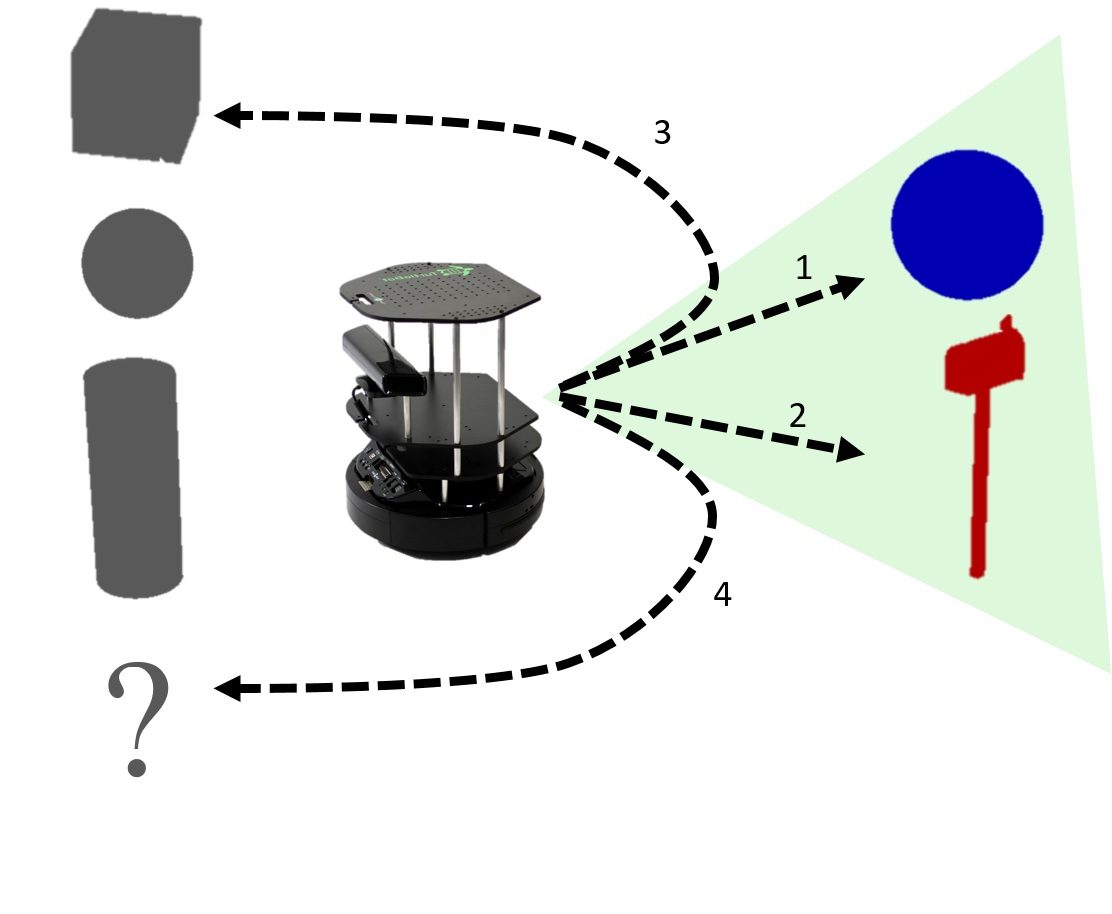
\includegraphics[width=8.5cm]{intro_pic}
	\caption{In this example, DCG-UPUP-Away has been trained only with cubes, spheres, and cylinders. DCG-UPUP-Away may ground phrases to known perceived objects (1), unknown perceived objects (2), known hypothesized objects (3), or unknown hypothetical objects (4).}
	\label{fig:intro_pic}
\end{figure}